\documentclass{article}

% if you need to pass options to natbib, use, e.g.:
%     \PassOptionsToPackage{numbers, compress}{natbib}
% before loading neurips_2019

% ready for submission
% \usepackage{neurips_2019}

% to compile a preprint version, e.g., for submission to arXiv, add add the
% [preprint] option:
    % \usepackage[preprint]{neurips_2019}

% to compile a camera-ready version, add the [final] option, e.g.:
\usepackage[final]{neurips}

% to avoid loading the natbib package, add option nonatbib:
    % \usepackage[nonatbib]{neurips_2019}
\usepackage{multicol}
\usepackage{float}
\usepackage[center]{caption}

\usepackage[utf8]{inputenc} % allow utf-8 input
\usepackage[T1]{fontenc}    % use 8-bit T1 fonts
\usepackage{hyperref}       % hyperlinks
\usepackage{url}            % simple URL typesetting
\usepackage{booktabs}       % professional-quality tables
\usepackage{amsfonts}       % blackboard math symbols
\usepackage{nicefrac}       % compact symbols for 1/2, etc.
\usepackage{microtype}      % microtypography
\usepackage{graphicx}
\usepackage{amsmath}
\usepackage{xepersian}

\settextfont{XB Yas.ttf}

\title{تکلیف شماره 3
 - 
 \lr{Leader Election}}


% The \author macro works with any number of authors. There are two commands
% used to separate the names and addresses of multiple authors: \And and \AND.
%
% Using \And between authors leaves it to LaTeX to determine where to break the
% lines. Using \AND forces a line break at that point. So, if LaTeX puts 3 of 4
% authors names on the first line, and the last on the second line, try using
% \AND instead of \And before the third author name.

\author{%
  امیرحسین مهدی‌نژاد\\
  شماره دانشجویی 810800058\\
  \texttt{mahdinejad@ut.ac.ir} \\
  % examples of more authors
  % \And
  % Coauthor \\
  % Affiliation \\
  % \texttt{email} \\
  % \AND
  % Coauthor \\
  % Affiliation \\
  % Address \\
  % \texttt{email} \\
}

% create title (includes both anonymized and non-anonymized versions)
% \providecommand{\@makepertitle}{}
% \newcommand{\makepertitle}{%
%   \vbox{%
%     \hsize\textwidth
%     \linewidth\hsize
%     \vskip 0.1in
%     \toptitlebar
%     \centering
%     {\LARGE\bf \@title\par}
%     \bottomtitlebar
%       \def\And{%
%         \end{tabular}\hfil\linebreak[0]\hfil%
%         \begin{tabular}[t]{c}\bf\rule{\z@}{24\p@}\ignorespaces%
%       }
%       \def\AND{%
%         \end{tabular}\hfil\linebreak[4]\hfil%
%         \begin{tabular}[t]{c}\bf\rule{\z@}{24\p@}\ignorespaces%
%       }
%       \begin{tabular}[t]{c}\bf\rule{\z@}{24\p@}\@author\end{tabular}%
%     \vskip 0.3in \@minus 0.1in
%   }
% }

\begin{document}


\begin{minipage}{0.1\textwidth}% adapt widths of minipages to your needs

\includegraphics[width=1.1cm]{Photos/UT_logo.png}
\end{minipage}%
\hfill%
\begin{minipage}{0.9\textwidth}\raggedleft
دانشکده فنی، دانشگاه تهران\\
سیستم‌های توزیع شده - 
آذر
ماه 1400\\
\end{minipage}
% \end{}

\makepertitle

% ----------------------------------------------------------------------

% \begin{abstract}
%  این بخش از یک پاراگراف تشکیل شده است که توضیحاتی کلی در مورد مساله و راه حل شما ارائه می‌دهد.
% \end{abstract}
\begin{multicols}{2}
\stepcounter{section}
\stepcounter{section}
\stepcounter{section}
\stepcounter{subsection}
\stepcounter{subsection}
\subsection{}
در الگوریتم پیشفرض
\lr{LCR}
رخ دادن 
\lr{halt}
در نظر گرفته نشده است. اما هنگامی که نود 
\lr{leader}
شماره‌ی خودش را دریافت می‌کند، با
\lr{broadcast}
کردن یک پیغام، رهبری خود را به رینگ اعلام می‌کند.\\
می‌توان الگوریتم را به صورت زیر تغییر داد:
\begin{figure}[H]
    \centering
    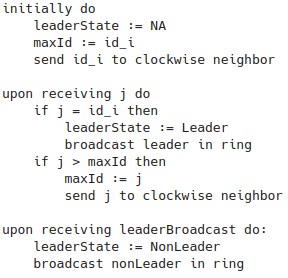
\includegraphics[width=0.95\linewidth]{Photos/HW3/lcr.png}
    \caption{
    در اینجا
    \lr{leaderState}
    یک متغیر سه حالته (یکی از حالات
    \lr{NA, Leader, NonLeader}
    ) است.
    }
    \label{fig:my_label}
\end{figure}
با توجه به بخش آخر این الگوریتم، هر نود وقتی از وجود
\lr{leader}
آگاه می‌شود، پیغام عدم رهبری خود را اعلام می‌کند. این ارسال پیام‌ها، در صورت سالم بودن ارتباطات، حداکثر به اندازه‌ی تعداد نودها طول می‌کشد و در نتیجه پیچیدگی زمانی تغییری نمی‌کند.\\
\rule{\linewidth}{1pt}

\subsection{}
در واقع ما با سیستم‌هایی سر و کار داریم که ممکن است نودها در 
\lr{round}
های مختلف اجرا شوند. در اینجا یک 
\lr{environment node}
تصور می‌شود که به همه‌ی نودهای دیگر یال داشته باشد و پیام‌های
\lr{wakeup}
برای آن‌ها ارسال کند. وضعیت آغازین نودها مگر در صورتی که این پیغام را برای بیداری دریافت کرده باشند یا پیغامی ناتهی از بقیه‌ی نودها رسیده باشد، به صورت پیشفرض 
\lr{quiescent}
یا خاموش است.\\
پس پیام‌ها به صورت همزمان ارسال نمی‌شوند ولی می‌خواهیم کل سیستم سنکرون باقی بماند، یعنی باید مکانیسمی طراحی کنیم که تا وقتی نودها هماهنگ نشدند، سراغ
\lr{round}
جدید نرویم. مثلاً می‌توان در کنار هر پیامی که ارسال می‌شود، مقداری را به عنوان شمارنده‌ی اینکه در کدام
\lr{round}
هستیم، رد و بدل کنیم. در نتیجه هر نود وقتی عددی را به عنوان شمارنده‌ی راند دریافت کند که کوچکتر از عددی باشد که خودش به عنوان راند می‌داند، نتیجه می‌گیرد که 
\lr{wakeup}
رخ داده است.\\
در واقع ماهیت الگوریتم تغییر خاصی نمی‌کند و نودها می‌توانند بدون توجه به اینکه نود دیگری ممکن است
\lr{quiescent}
باشد، به کار خود ادامه دهند.\\
\rule{\linewidth}{1pt}

\stepcounter{subsection}
\stepcounter{subsection}
\stepcounter{subsection}
\stepcounter{subsection}
% \subsection{}

\subsubsection{}
فرض کنیم حالتی در 
\lr{ring}
داشته باشیم که نودها به ترتیب نزولی
\lr{id}
ها در جهت عقربه‌های ساعت قرار گرفته باشند. در این حالت اگر جهت ارسال پیام نیز در جهت عقربه‌های ساعت باشد،
در اولین راند فقط و فقط یک نود حذف می‌شود. به همین ترتیب برای محاسبه‌ی پیچیدگی پیامی داریم:
$$2.(n + 2.(n-1) + 4.(n-2) + \dots$$
$$ + 2^{\log{n}}.(n-2^{\log{n}-1}))$$
$$=2.\left(\dfrac{2}{3}.(4^{\log{n}}-1) + (2^{\log{n}+1}-1).n\right)$$
$$\in \mathcal{O}(n^2)$$
در صورتی که اگر ارسال پیام دو طرفه بود، چنین حالتی مشکل‌ساز نمی‌شد، چرا که هر نود به نودهای راست و چپ خود پیغام می‌فرستاد و در هر راند نودهای باقی‌مانده نصف می‌شدند.
\begin{figure}[H]
    \centering
    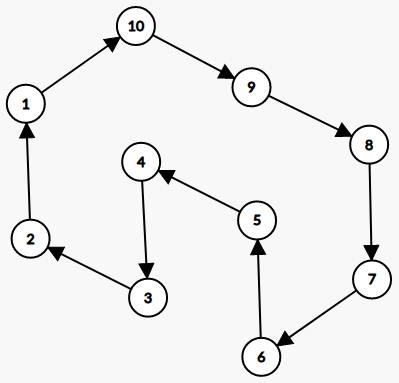
\includegraphics[width=0.95\linewidth]{Photos/HW3/cycle.png}
    \caption{
    نمونه‌ای از حلقه‌ی نامطلوب برای الگوریتم
    \lr{HS}
    یک‌طرفه، به ازای ۱۰ نود
    }
    \label{fig:my_label}
\end{figure}

\subsubsection{}
مزیت ارسال پیام به دو طرف این بود که مطمئن می‌شدیم یکی از طرفین راست یا چپ بالاخره در هر بار ارسال پیام، متوجه می‌شوند که 
\lr{leader}
نیستند. الآن با توجه به اینکه فقط نودها به یک سمت می‌توانند پیام ارسال کنند می‌توانیم آن مزیت را به نحوی بازسازی کنیم. اگر نودهای توپولوژی یک در میان به صورت
\lr{clockwise}
و یا
\lr{counterclockwise}
پیام بفرستند، در واقع در هر راند نود کوچکتری که توسط نود
\lr{i}
ام حذف نشده باشد، توسط یکی از همسایه‌های این نود حذف شده است.\\
لذا هیچ چینش 
\lr{id}
خاصی وجود ندارد که به ازای آن، یک نود
\lr{nonLeader}
بتواند مانند حالتی که در بند قبلی این سوال رخ داد، از حذف شدن جان سالم به در ببرد.\\
گرچه تعداد مراحل یا
\lr{round}
های الگوریتم در هر دو روش (یک‌طرفه و دوطرفه) یکسان بود، اما برتری روش دوطرفه در حذف شدن نودهای بیشتر برای مرحله‌ی بعد بود. در واقع همان‌طور که در توضیحات بند قبل اشاره شد، نودهای
\lr{nonLeader}
به علت مقایسه شدن با نودهای کوچکتر (در ترتیب نزولی) تا مدت زیادی حضور داشتند در صورتی که اگر بجای همسایه‌ی سمت راستی به همسایه‌ی سمت چپی پیام می‌دادند، همان سری اول می‌فهمیدند که رهبر نیستند.

\end{multicols}
\end{document}
